\chapter{Descripción de la aplicación}
% La aplicación MiApp
TransDrakkar es una aplicación web para gestionar el transporte de mobiliario desde la solicitud del cliente hasta la entrega. El estado descrito corresponde al cierre del Sprint 2, a 17 de noviembre de 2026. El incremento incluye perfiles de cliente, administrador y conductor, revisión de solicitudes, recursos, rutas y seguimiento de entregas. La confirmación de correo y el acceso con Google cuentan con implementación y pruebas simuladas; se distingue ese alcance de la validación real de los proveedores.

\section{Requisitos}
% Una lista (requisitos funcionales, no funcionales...) / O algo mas eleborado (stakeholders, técnica personas)
\subsection{Requisitos funcionales}
\begin{itemize}
\item RF-01. Registrar una cuenta con correo y contraseña, evitando correos duplicados.
\item RF-02. Confirmar la cuenta mediante un enlace de un solo uso y permitir solicitar un nuevo enlace.
\item RF-03. Iniciar y cerrar sesión, y recuperar la sesión al recargar mientras siga vigente.
\item RF-04. Permitir el acceso con una cuenta de Google con correo verificado.
\item RF-05. Distinguir los permisos de usuario y administrador. El administrador puede listar usuarios y consultar su estado.
\item RF-06. Permitir al usuario eliminar su cuenta y al administrador eliminar otras cuentas. Una cuenta eliminada no debe poder acceder.
\item RF-07. Mostrar al usuario mensajes ante errores de validación, acceso, red y servicios externos.
\item RF-08. Presentar el acceso con la identidad visual de TransDrakkar (requisito de interfaz, P15).
\item RF-09. Proporcionar paneles y permisos de cliente, conductor y administrador (P16).
\item RF-10. Crear solicitudes con recogida y entrega completas, mercancía, fecha e idempotencia (P17).
\item RF-11. Consultar las solicitudes propias, su estado y su historial.
\item RF-12. Cancelar solicitudes propias mientras estén pendientes, conservando su historial.
\item RF-13. Revisar solicitudes desde administración, aceptar o rechazar con motivo (P19).
\item RF-14. Gestionar vehículos activos y disponibles para planificar (P21).
\item RF-15. Gestionar conductores vinculados a cuentas habilitadas (P21).
\item RF-16. Planificar rutas desde Yecla y asignar vehículo, conductor y paradas ordenadas sin conflictos (P22).
\item RF-17. Consultar el itinerario propio y registrar entregas o incidencias autorizadas (P23).
\end{itemize}
\subsection{Requisitos no funcionales}
Las contraseñas se almacenan mediante hashes bcrypt. Los permisos se comprueban en el servidor y las cuentas persisten en MongoDB. La aplicación se organiza por capas para facilitar el mantenimiento y dispone de pruebas automatizadas. La configuración sensible se suministra mediante variables de entorno y secretos externos al repositorio.

\section{Arquitectura de la solución}
La solución sigue una arquitectura por capas. El navegador presenta la interfaz; el cliente HTTP invoca una API REST; la lógica aplica las reglas de negocio y la capa de datos accede a MongoDB.

La Figura~\ref{fig:arquitectura-capas} resume esta organización: el cliente se ejecuta en el navegador y se comunica con el servidor, organizado en API, lógica y datos. La capa de datos accede al servicio de base de datos. El nombre \texttt{mi\_bbdd} del esquema es ilustrativo; en la implementación descrita se utiliza MongoDB Atlas.
\begin{figure}[htbp]
\centering
\includegraphics[width=0.95\textwidth]{figs/arquitectura-capas.png}
\caption{Esquema de organización de la aplicación: cliente web, servidor por capas y servicio de base de datos.}
\label{fig:arquitectura-capas}
\end{figure}

\begin{description}
\item[Presentación.] La carpeta \texttt{cliente} contiene la página HTML, los estilos CSS y el módulo JavaScript de presentación que define el comportamiento de la interfaz.
\item[Comunicación.] \texttt{cliente/rest.js} centraliza las peticiones HTTP.
\item[API.] \texttt{servidor/api.js} define las rutas y respuestas HTTP con Express.
\item[Lógica.] \texttt{servidor/logica.js} implementa validaciones, autenticación y autorización.
\item[Persistencia.] \texttt{datos.js} selecciona el adaptador de datos. MongoDB conserva cuentas, sesiones, solicitudes, recursos y rutas; SQLite se reserva para pruebas aisladas.
\item[Servicios auxiliares.] \texttt{sesiones.js}, \texttt{externos.js} y \texttt{correo.js} gestionan sesiones, acceso con Google y correo de confirmación.
\end{description}
El contenedor de Cloud Run sirve tanto el cliente como el servidor, mientras que MongoDB Atlas almacena los datos de acceso y transporte. El código de acceso con Google utiliza Authorization Code con PKCE y el correo se envía mediante SMTP. Ambos servicios necesitan sus credenciales y una comprobación real antes de considerarse completados.
En la revisión actual, las sesiones duran ocho horas y se almacenan en MongoDB Atlas, junto con el identificador de usuario y la fecha de caducidad. El navegador conserva una cookie de acceso; reiniciar el servidor no elimina una sesión vigente. Esta descripción actualiza la limitación de la versión anterior, que utilizaba memoria del proceso.

\clearpage
\subsection{Diagrama de despliegue}
La Figura~\ref{fig:despliegue-transdrakkar} muestra la distribución de TransDrakkar entre los dispositivos de acceso y los servicios que ejecutan la aplicación. Complementa la vista por capas anterior: representa dónde se ejecuta el software y los protocolos que conectan sus nodos.

\begin{center}
\begin{minipage}{\textwidth}
\centering
\includegraphics[width=\textwidth]{figs/despliegue-persistente.png}
\captionsetup{hypcap=false}
\captionof{figure}{Diagrama de despliegue de TransDrakkar: navegador, aplicación en Cloud Run, persistencia en Atlas y servicios externos.}
\label{fig:despliegue-transdrakkar}
\end{minipage}
\end{center}

El usuario accede desde un navegador en un ordenador o teléfono mediante HTTPS. Google Cloud Run ejecuta un contenedor Docker con Node.js y Express que sirve los archivos del cliente y la API REST. La base de datos se aloja fuera del contenedor, en MongoDB Atlas, y la comunicación utiliza TLS. En la evolución del Sprint 2, el almacenamiento contempla usuarios, solicitudes de recogida y rutas; el cierre del Sprint 2 incorpora el recorrido completo de solicitud, revisión, planificación y entrega, con historial y permisos por perfil.

Google OAuth/OpenID Connect interviene en el acceso con Google y Gmail SMTP en el envío de los enlaces de confirmación. El diagrama representa las integraciones previstas en el código; su aparición no acredita que estén configuradas y verificadas en producción. Las sesiones se conservan en Atlas y sobreviven al reinicio del servidor hasta su caducidad o invalidación. El máximo de una instancia sigue siendo la configuración de despliegue documentada; no se afirma que el escalado de todo el sistema esté validado, pues aunque el estado de OAuth ya persiste en Atlas, los límites de acceso son por proceso y requieren revisión antes de ampliar instancias.

\subsection{Diagrama de secuencia: acceso del Sprint 1}
La Figura~\ref{fig:secuencia-login} representa el inicio de sesión con correo y contraseña, un caso de uso de la gestión de acceso del Sprint 1. Se utiliza la implementación actual para explicar la colaboración entre interfaz, API, lógica y persistencia. El almacenamiento de sesiones en MongoDB es una mejora de la revisión actual; este esquema no atribuye su fecha de implementación al cierre del Sprint 1.

\begin{center}
\begin{minipage}{\textwidth}
\centering
\includegraphics[width=\textwidth,height=0.78\textheight,keepaspectratio]{figs/secuencia-login.png}
\captionsetup{hypcap=false}
\captionof{figure}{Inicio de sesión con correo y contraseña y recuperación de una sesión vigente. Caso de uso del Sprint 1 representado con la persistencia de la revisión actual.}
\label{fig:secuencia-login}
\end{minipage}
\end{center}

El usuario introduce sus credenciales y la interfaz envía una petición de acceso a la API. La lógica normaliza y valida los datos, busca la cuenta y compara la contraseña con su hash mediante bcrypt. Una cuenta inexistente o eliminada, una contraseña incorrecta o una cuenta pendiente de confirmar impiden crear la sesión y producen una respuesta de autenticación fallida. La contraseña y su hash no se devuelven al navegador.

Si la cuenta puede acceder, el servidor genera un token aleatorio y guarda en la base de datos su hash SHA-256, el identificador del usuario y la caducidad de ocho horas. El navegador recibe el token en una cookie HttpOnly, con Secure en producción, y la respuesta contiene los datos públicos de la cuenta. La persistencia es invocada por el módulo de sesiones; el diagrama agrupa esos detalles internos para facilitar la lectura.

Al recargar la página, la interfaz consulta la sesión con la cookie. El servidor recupera una sesión no caducada y vuelve a comprobar la cuenta antes de permitir el acceso. Un reinicio de Cloud Run no elimina las sesiones almacenadas en Atlas. Se requiere que la cookie siga disponible, la sesión no haya caducado ni se haya cerrado y la cuenta continúe autorizada. Conservar una cuenta registrada y conservar una sesión autenticada son responsabilidades distintas; ambas disponen de persistencia en el código actual.

\clearpage
\subsection{Diagrama de secuencia: solicitud de recogida}
La Figura~\ref{fig:secuencia-recogida} describe el caso de uso de creación de una solicitud de recogida en fábrica, incorporado en el PBI P17 del Sprint 2. Esta vista amplía la descripción de gestión de cuentas de octubre con el comportamiento incorporado en P17 y conservado en la revisión de cierre del Sprint 2. Participan el cliente, la interfaz web, la API REST, la lógica de solicitudes y MongoDB Atlas. Las líneas discontinuas representan respuestas y los bloques \texttt{alt} distinguen los resultados alternativos.

\begin{center}
\begin{minipage}{\textwidth}
\centering
\includegraphics[width=\textwidth,height=0.80\textheight,keepaspectratio]{figs/secuencia-recogida.png}
\captionsetup{hypcap=false}
\captionof{figure}{Secuencia de creación de una solicitud de recogida, con autorización, validación y prevención de envíos duplicados.}
\label{fig:secuencia-recogida}
\end{minipage}
\end{center}

\begin{sloppypar}
El recorrido parte de un cliente con sesión iniciada que completa el fabricante, la dirección y el contacto de recogida, la fecha, las líneas de mercancía y los datos completos de destinatario, dirección y contacto de entrega. La interfaz envía una petición \texttt{POST} a \texttt{/api/solicitudes} con los datos, la cookie de sesión y una cabecera \texttt{Idempotency-Key}. La API comprueba la sesión y consulta la cuenta para verificar que está confirmada, activa y tiene perfil de cliente. El propietario se obtiene de la identidad autenticada; el navegador no decide a qué cuenta se asigna la solicitud.
\end{sloppypar}

La lógica valida los datos y la fecha y solicita el guardado a través de la capa de persistencia, resumida en el diagrama junto a MongoDB para facilitar la lectura. El servidor fija el identificador, la referencia y el estado inicial \texttt{pendiente\_recogida}. Una creación correcta devuelve \texttt{201 Created}. Si se repite la misma clave con los mismos datos, se recupera la solicitud existente y se responde \texttt{200 OK}; un índice único por cliente y clave evita duplicados incluso con peticiones concurrentes. Reutilizar la clave con datos diferentes produce \texttt{409 Conflict}.

Los datos inválidos generan \texttt{400 Bad Request} y una cuenta sin el perfil requerido recibe \texttt{403 Forbidden}. La precondición del esquema es una sesión válida; la ausencia de autenticación se rechaza antes del caso de uso. La interfaz presenta el resultado y conserva los datos ante errores. Esta operación registra la petición de recogida; la asignación de conductores y la planificación posterior se desarrollan en otros casos de uso.


\clearpage
\subsection{Diagrama de estados del transporte}
El diagrama de la Figura~\ref{fig:estados-transporte} resume el ciclo de cada solicitud y las transiciones permitidas al cerrar el Sprint 2. Complementa la secuencia de alta con los casos de revisión, planificación y entrega. El estado de la ruta agrupa el resultado de sus paradas: una incidencia abierta no libera reservas ni completa la ruta.
\begin{center}
\begin{minipage}{\textwidth}
\centering
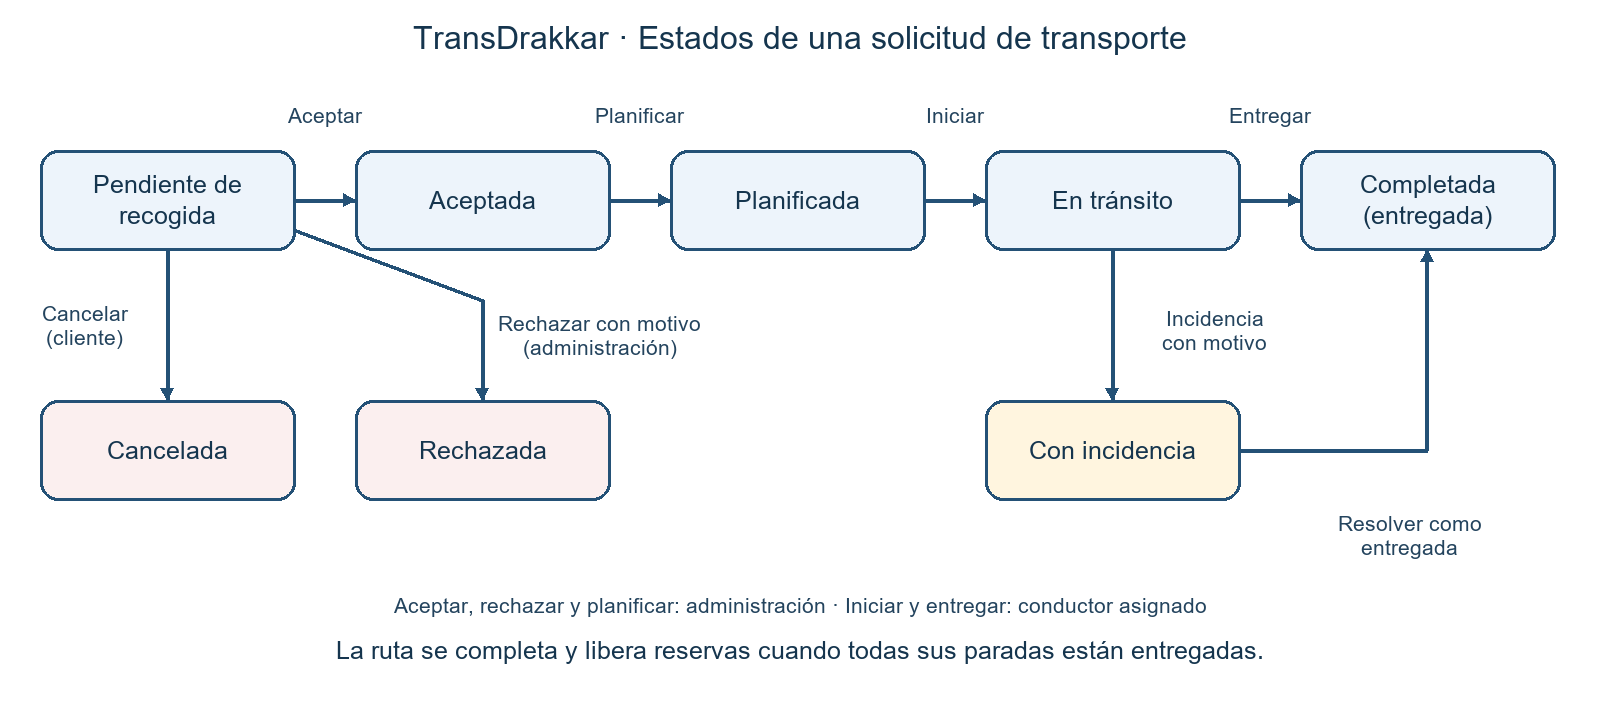
\includegraphics[width=0.95\textwidth,height=0.48\textheight,keepaspectratio]{figs/estados-transporte-sprint2.png}
\captionsetup{hypcap=false}
\captionof{figure}{Estados de la solicitud y acciones autorizadas por perfil. La ruta solo se completa cuando todas sus paradas están entregadas.}
\label{fig:estados-transporte}
\end{minipage}
\end{center}

El cliente solo cancela una solicitud pendiente. Administración acepta o rechaza con motivo y planifica las aceptadas. El conductor asignado inicia la ruta y comunica entregas o incidencias; una incidencia exige motivo y puede resolverse como entrega. No se permiten retornos desde un estado final. Las claves idempotentes y revisiones evitan duplicados y sobrescrituras, mientras las transacciones mantienen consistentes solicitudes, paradas y ruta.

\section{Desarrollo del Proyecto}
El Anexo~\ref{anexo:desarrollo} conserva la revisión histórica del Sprint 1 y desarrolla el cierre del Sprint 2. Este segundo incremento añade el proceso de transporte completo a la base de acceso. Los ocho PBI presentes en las capturas suman 50 de estimación visible y 26,8 horas registradas. Se separan ambas magnitudes porque la unidad de estimación no está confirmada en las capturas. El anexo explica las discrepancias con los gráficos de seguimiento de DoneTonic.

\section{TransDrakkar: guía de uso}
\subsection{Registro, confirmación y acceso}
Crear cuenta solicita nombre, primer apellido, correo y contraseña. La cuenta pública recibe perfil cliente y queda pendiente de confirmar el correo. La contraseña tiene un mínimo de seis caracteres y un máximo de 72 bytes; se almacena mediante bcrypt. El enlace de confirmación caduca a las 24 horas y es de un solo uso. Si el envío falla, el servicio informa del resultado y permite reintentar. El acceso con Google utiliza correo verificado y no vincula una cuenta local solo por coincidencia de dirección. La aplicación recupera sesiones vigentes al recargar y permite cerrarlas.

\subsection{Cliente: solicitud y seguimiento}
El cliente crea una solicitud con fabricante, origen en Yecla, contacto y fecha de recogida, mercancía y entrega final completa. Puede consultar solo sus solicitudes y abrir su detalle e historial. Mientras siguen pendientes puede cancelarlas. Un rechazo administrativo muestra su motivo. Durante la ejecución ve los estados en tránsito, incidencia y completada y los motivos registrados. Los datos antiguos incompletos se conservan y no se completan automáticamente.

\subsection{Administración: recursos y planificación}
Administración revisa y filtra solicitudes, acepta o rechaza con motivo y habilita cuentas de conductor. El catálogo guarda vehículos con matrícula única normalizada, capacidad con unidad, sede, actividad y disponibilidad; los conductores se vinculan a cuentas activas sin duplicarlas. Se conservan registros históricos al desactivar recursos.

Desde Planificar rutas se elige fecha, camión y conductor disponibles en Yecla y de 1 a 100 solicitudes aceptadas distintas. Se ordenan las paradas antes de guardar. Una solicitud no puede pertenecer a dos rutas activas y un vehículo o conductor no se reserva dos veces en la misma fecha. El itinerario permite revisar direcciones, contactos, mercancía y seguimiento de cada parada.

\subsection{Conductor: itinerario, entregas e incidencias}
El conductor pulsa Ver ruta y entregas en una ruta asignada. Se muestran paradas en orden, dirección, contactos y mercancía. Iniciar ruta pasa sus solicitudes a en tránsito. Cada parada permite Marcar entregada o Registrar incidencia con motivo obligatorio. Resolver como entregada cierra una incidencia; la última entrega completa la ruta y libera sus reservas. Solo se confirma éxito tras respuesta del servidor; un fallo de red ofrece reintentar sin duplicar el evento. Las rutas previas con itinerario completo también pueden ejecutarse.

\section{Pruebas y validación}
La ejecución CI \href{https://github.com/Miguel-Requena/Procesos26-27/actions/runs/44078563639}{44078563639 del PR 42} contiene 85 casos, sin fallos ni omisiones, e incluye MongoDB real con replica set y comprobación del contenedor. El artefacto JUnit conserva los resultados. La regresión local supera 83 casos y omite las dos integraciones MongoDB si no hay instancia disponible; se distingue ese resultado del remoto.

Las pruebas cubren autenticación y permisos, propiedad, fechas inválidas, duplicados, estados, revisiones obsoletas, concurrencia, rollback, persistencia entre procesos y liberación de reservas. El escenario T34 recorre por HTTP solicitud, aceptación, ruta, incidencia, entrega y consulta cliente. T35 comprueba negativos y reintentos tras perder la respuesta. La prueba visual con dos paradas ficticias comprueba la ejecución y su historial. El anexo de desarrollo identifica entradas y evidencias sin modificar operaciones reales de producción.

Las pruebas de correo y Google utilizan proveedores simulados y no acreditan recepción real o consentimiento. La persistencia comprobada entre procesos tampoco se presenta como reinicio manual de Cloud Run. Estos límites no deben confundirse con funciones de transporte pendientes.

\section{Despliegue y estado actual}
La aplicación se publica en \href{https://procesos26-27-gseerr4ika-no.a.run.app}{Google Cloud Run}, con MongoDB Atlas. Las ramas específicas y PR con CI satisfactoria se integran en main; Cloud Build construye y despliega automáticamente el contenedor. El cierre P23/P24 se integra mediante el \href{https://github.com/Miguel-Requena/Procesos26-27/pull/42}{PR 42}, commit de integración \texttt{885b380}. Se verificó disponibilidad de la interfaz desplegada de entregas y rechazo 401 de la API operativa sin sesión. Las credenciales se mantienen fuera del repositorio y de la memoria.
